\documentclass[8pt,a9paper]{beamer} \usepackage[utf8]{inputenc} \usepackage[francais]{babel} \usepackage[T1]{fontenc}
\usepackage{amsmath} \usepackage{amsfonts} \usepackage{amssymb} \usepackage{tikz} \usepackage{colortbl}
\title{Applications du Théorème de Superposition de Kolmogorov à la compression d'images} \date{}
\author{Nicolas Lebbe}
\author{Félix Piédallu}
\setlength{\unitlength}{1mm}
\usetheme{Boadilla}
\useoutertheme{Tipe} \setbeamerfont{headline}{size=\small}
%\setbeamertemplate{itemize subitem}[circle] 
\newcommand{\titp}[1]{\begin{center}\large{\textbf{#1}}\end{center}}
\newcommand{\image}[3]{\begin{tabular}{c}\includegraphics[#1]{#2}\\ #3 \end{tabular}}
\definecolor{vertpale}{rgb}{0.7, 0.9, 0.3}
\definecolor{jaunepale}{rgb}{1, 0.95, 0.41}
\definecolor{rougepale}{rgb}{0.77, 0.3, 0.32}
\begin{document}

\begin{frame}
	\maketitle
	\hspace{3cm}I. \textbf{{\large Introduction}}\textbf{\\}\textbf{\\}
	\hspace{2.9075cm}II. \textbf{{\large Le Théorème de superposition de Kolmogorov}}\textbf{\\}\textbf{\\}
	\hspace{2.815cm}III. \textbf{{\large L'application à la compression d'images}}\textbf{\\}\textbf{\\}
\end{frame}
\section{Introduction}
\subsection{Le Problème de la Dimension}
\begin{frame}
\titp{Introduction}
	\begin{columns}[t]
	\begin{column}{6.4cm}
		\begin{center}\emph{En Physique :}\end{center}
		\begin{itemize}
		\item \textbf{Problème de Navier-Stokes}
		\begin{description}
		\item[Dimension 2 :] Résolu (Jean Leray, 1934)
		\item[] 
		\item[]	
		\item[Dimension 3 :] 6\ieme  Problème du Millénaire
		\item[] 
		\item[] 
		\end{description}
		\item \textbf{Le problème à n corps}
		\begin{description}
		\item[2 corps :] Solutions énoncées \\ Isaac Newton (1687)
		\item[]	
		\item[3 corps :] 1909 (Karl Sundman) : résultats, mais inutilisables.
		\item[$\rightarrow$] Théorie du Chaos (incertitude)
		\end{description}
		\end{itemize}
	\end{column}
	\begin{column}{6.4cm}
		\begin{center}\emph{En Mathématiques :}\end{center}
		\begin{itemize}
		\item \textbf{Solutions d'équations polynômiales}
		\begin{description}
		\item[Degré inférieur à 4 :] Formules exactes\\ par radicaux
		\item[]	
		\item[Degré supérieur :] Pas de solutions analytiques (É. Galois, \uppercase\expandafter{\romannumeral 18}\ieme).
		\item[] 
		\end{description}
		\item \textbf{Le Théorème de Fermat : $a^n+b^n=c^n$}
		\begin{description}
		\item[Pour n=2 :] Théorème de Pythagore (Antiquité)
		\item[]	
		\item[Pour n>2 :] Impossible d'après A.Wiles (1994)
		\item[$\rightarrow$] Topologie algébrique
		\end{description}
		\end{itemize}
	\end{column}
	\end{columns} 
\end{frame}
	%\begin{frame}
	%	\begin{block}{Treizième problème de David Hilbert :}
	%	"Montrer l'impossibilité de résoudre les équations du septième degré au moyen de fonctions de \alert{seulement deux variables},\\cela étant pourtant vrai avec 3 variables."
	%	\end{block}
	%	\begin{center}$\Leftrightarrow$ \end{center}
	%	\begin{center}Reformulation de Hilbert :\end{center}
	%	\[\exists f \in C^o([0,1]^3) \;;\; \nexists \; k,h,g \in C^o([0,1]^2), \forall (x,y,z) \in [0,1]^3, \; f(x,y,z)=k(h(x,y),g(y,z)) \]
	%	\newline
	%	En 1957, V. Arnold  réfute ceci par le cas $n=3$ du Théorème de Kolmogorov, qui est étendu peu après à tout $n \in \mathbb{N}$.
	%\end{frame}
\subsection{L'énoncé du Théorème} %%%%%%%%%%%%%%%%%%%%%%%%%%%%%%%%%%%%%%%%%%%%%%%%%%%%%%%%%-------------------------- À changer
\begin{frame}
	\begin{block}{Le Théorème de Superposition de Kolmogorov}
	$ \forall n \in \mathbb{N}^* , \exists \left\lbrace \begin{array}{l} \lambda_1 ,…, \lambda_n \in \mathbb{R}^* \text{de somme 1}\\ \phi_1,…, \phi_{2n+1} \in \mathcal{C}^0([0,1])\end{array} \right. $ \underline{universels} \textbf{telles que}\\
	\textbf{\\}
	Pour $ f \in \mathcal{C}^o([0,1]^n, \mathbb{R})$ \emph{quelconque},\\
	\begin{center} $\exists g_1,…,g_{2n+1}\in \mathcal{C}^o (\mathbb{R},\mathbb{R})$, dépendantes de f, \textbf{telles que} \end{center}
	\[f(x_1,…,x_n)= \sum\limits_{q=1}^{2n+1} g_q\left(\sum\limits_{p=1}^{n}\lambda_p\phi_q(x_p)\right) \]
	\end{block}
	Ceci représente toute fonction à n variables comme somme de composées de fonctions à une variable.\\
	\textbf{\\}
	Par exemple, il existe $\left\lbrace \begin{array}{l} \lambda_a ,…, \lambda_c \\ \phi_1,…,\phi_5 \end{array} \right.$, tels que : \begin{itemize}
	\item[•] Pour tout $(x,y,z) \in [0,1]^3$, $\sqrt{\cos^2(xy)+z} = \sum\limits_{q=1}^{7} g_q\left(\lambda_a\phi_q(x)+\lambda_b\phi_q(y)+\lambda_c\phi_q(z) \right)$
	\item[•] Pour tout $(x,y,z) \in [0,1]^3$, $e^{x\sin(z-y)} = \sum\limits_{q=1}^{7} h_q\left(\lambda_a\phi_q(x)+\lambda_b\phi_q(y)+\lambda_c\phi_q(z)\right)$
	\end{itemize}
\end{frame}
\section{Le Théorème de Superposition de Kolmogorov}
\subsection{Quelques prérequis mathématiques}
\begin{frame}
	\begin{block}{Le Théorème de Baire}
	Soit E un espace vectoriel normé complet (Banach) et $(O_n)_n$ une suite d'ouverts denses de E.
	\begin{center}
	Alors $\bigcap_{n \in\mathbb{N}} O_n$ est dense dans E.
	\end{center}
	\end{block}
	\textbf{\\}
	\begin{exampleblock}{}
	\textbf{Déf : }P est vraie pour \textbf{quasi tout} $x \in E$, si P est vraie sur une intersection d'ouverts denses dans E (notée un $G_\delta$-dense)
	\end{exampleblock}
	\textbf{\\}
	\begin{exampleblock}{}
	\textbf{Déf : }$\Phi$ est l'ensemble des fonctions $\varphi$ strictement croissantes, continues sur $I$, telles que $\varphi(0)=0 , \varphi(1)=1$.\\
	Muni de $\|\|_\infty$, c'est un espace métrique complet
	\end{exampleblock}
\end{frame}
\subsection{La Preuve non-constructive du Théorème.}
\begin{frame}
	\titp{Preuve non-constructive du Théorème de Kolmogorov :}
	\textbf{\\}
	\textbf{\\}

	Soit $\rho \in \mathcal{C}^o([0,1]^n, \mathbb{R})$, et $\lambda_1,…,\lambda_n$ strictement positifs de somme $1$.\\
	Soit $\epsilon>0$. \\\textbf{\\}
	Définissons $\Omega(f)=\left\lbrace (\varphi_1,…, \varphi_{2n+1}) \in \Phi^{2n+1} \text{ tel qu'il existe } h \in C(I^n)\right\rbrace$ avec $\|h\|_\infty \leq \|f\|_\infty$ et\\	\textbf{\\}
	\begin{equation}
	\displaystyle \left\| f(x_1,…, x_n) - \sum_{q=1}^{2n+1} h \left(\sum_{p=1}^n \lambda_p \varphi_q (x_p) \right) \right\|_\infty < (1-\epsilon)\|f\|_\infty \label{Th}
	\end{equation}
	\textbf{\\}	\textbf{\\}
	\textbf{\\}	\textbf{\\}
	$\Omega(f)$ est un ouvert de $\Phi ^{2n+1}$, admis dense. \\
	\textbf{\\}
	Soit F un ensemble dénombrable dense dans $C(I^n)\backslash\{0\}$.\\
	$\bigcap_{f \in F} \Omega(f)$ est dense dans $\Phi^{2n+1}$ : c'est une intersection dénombrable d'ouverts denses dans $E$.\\
	On y prend $(\varphi_1,…,\varphi_{2n+1})$.\\
	\textbf{\\}
\end{frame}
\begin{frame}
	Il existe $f_0 \in F$, telle que
		$\left\lbrace \begin{array}{ccc} \|f_0\|_\infty &\leqslant &\|\rho\|_\infty \\ \|\rho-f_0\|_\infty &<&\frac{\epsilon}{2} \|\rho\|_\infty\end{array} \right.$
		et $h_0$ vérifiant $(1)$ pour $f_0$.\\
	\textbf{\\}
	\textbf{\\}
	Notons $h_0= \gamma(f_0)$, et $\gamma(0)=0$.\\
	\textbf{\\}
	Par récurrence, nous définissons $h_j = \gamma(f_j)$, et
	\begin{equation} \label{Termesérie}
	f_{j+1}(x_1,…,x_n)= f_j(x_1,…, x_n) - \sum_{q=1}^{2n+1} h_j\left( \sum_{p=1}^n \lambda_p \varphi_q(x_p)\right)
	\end{equation}
	Or $\displaystyle \lim_{j \to +\infty} \|f_j\|_\infty = 0$. On peut sommer par télescopage.\\
	\textbf{\\}
	\textbf{\\}
	La série $\sum_{j=0}^\infty h_j$ converge dans $C(I)$ vers $g$ qui vérifie alors, comme (\ref{Th}) a lieu, le théorème pour $f_0$.\\
\end{frame}

\section{L'application à la compression d'images}
\subsection{Le principe}
\begin{frame}
	\titp{Application aux images :}
	\textbf{\\}
	\begin{center}
	\begin{minipage}[c]{4cm}
	\begin{center}
	$\overbrace{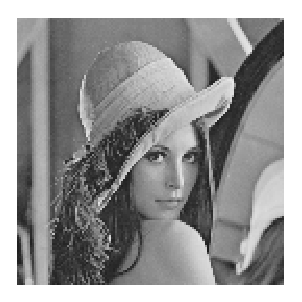
\includegraphics[scale=0.8]{lena.eps}}^{\text{n pixels (128)}}$\\
	Image originale\\Fonction discrète\\
	$n^2$ points à enregistrer
	\end{center}
	\end{minipage}
	$\xrightarrow[\text{Interpolation linéaire}]{}$
	\begin{minipage}[c]{4cm}
	\begin{center}
	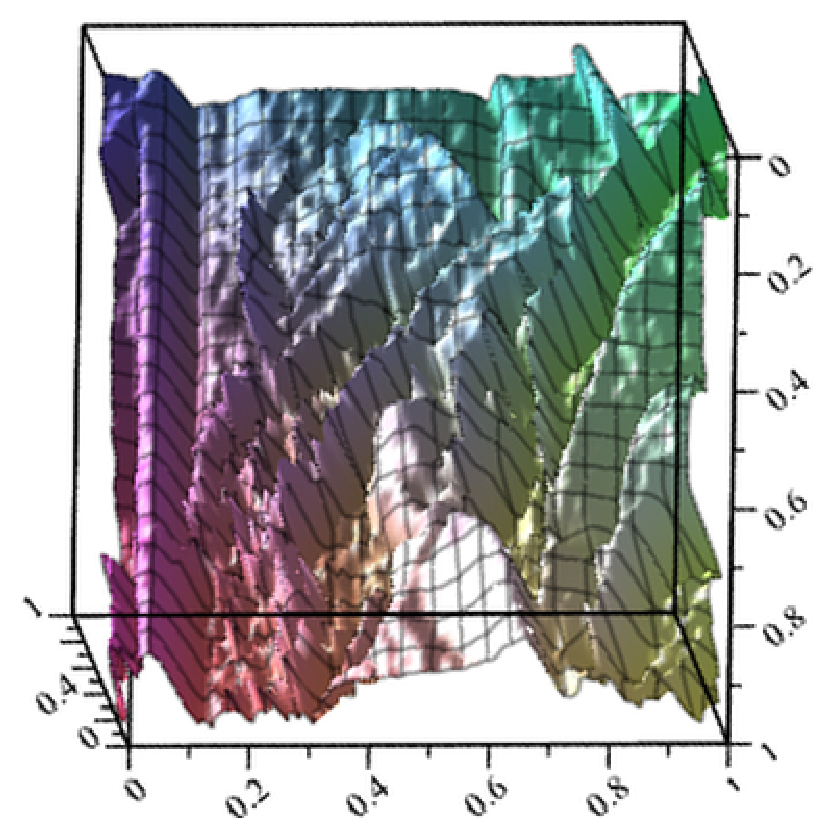
\includegraphics[scale=0.27]{lena3d.eps}\\
	Fonction $f$ continue sur $[0,1]^2$ \\
	Fonction superposable\\ par le théorème de Kolmogorov.
	\end{center}
	\end{minipage}
	\end{center}
	Un pixel repéré par $(x,y)$ est associé au point $({x\over n},{y\over n}) \in [0,1]^2$.
\end{frame}
\begin{frame}
	\titp{ Le théorème dans le cas des images : }
$\displaystyle f(x,y)=\sum_{n=0}^4 g_n(\underbrace{\lambda_1 \cdot \phi(x+n b)+\lambda_2\cdot \phi(y+n b)}_{\xi(x+n b, y + n b)}) \Rightarrow$
	\begin{minipage}[c]{5cm}
	\begin{tikzpicture}[thick,scale=0.7, every node/.style={scale=0.7},ultra thin,>=latex]
		\node[draw=black] (x) at (0,0) {\tiny{x}};
		\node[draw=black, minimum width=35] (phi1x) at (2,1) {\tiny{$\phi(x)$}};	\draw[->] (x) -- (phi1x.west);
		\node at (2,0.5) {$\cdots$};
		\node[draw=black, minimum width=35] (phi4x) at (2,0) {\tiny{$\phi(x+4b)$}};	\draw[->] (x) -- (phi4x.west);
		\node[draw=black] (y) at (0,-1) {\tiny{y}};
		\node[draw=black, minimum width=35] (phi1y) at (2,-1) {\tiny{$\phi(y)$}};	\draw[->] (y) -- (phi1y.west);
		\node at (2,-1.5) {$\cdots$};
		\node[draw=black, minimum width=35] (phi4y) at (2,-2) {\tiny{$\phi(y+4b)$}};	\draw[->] (y) -- (phi4y.west);
		\node[draw=black, minimum width=35] (g0) at (5,0) {\tiny{$g_0(\xi(x+0 b, y + 0 b))$}};
			\draw[->] (phi1x.east)-- (g0.north west) ; \draw[->] (phi1y.east)-- (g0.south west) ;
		\node at (5,-0.5) {$\cdots$};
		\node[draw=black, minimum width=35] (g4) at (5,-1) {\tiny{$g_4(\xi(x+4b, y + 4b))$}};
			\draw[->] (phi4x.east)-- (g4.north west) ; \draw[->] (phi4y.east)-- (g4.south west) ;
		\node[draw=black, minimum width=35] (fonction) at (7,-0.5) {$f(x,y)$};
			\draw[->] (g0.east) -- (fonction.west) ; \draw[->] (g4.east)-- (fonction.west) ;
	\end{tikzpicture}
	\end{minipage}\\
	
	\begin{center}	\end{center}\begin{center}	\end{center}
	\begin{center}
	\begin{minipage}[c]{2.3cm}\begin{center}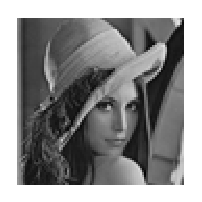
\includegraphics[scale=0.7]{SprecherPics/Originale.eps}\\Image Originale\\ \textbf{ } \end{center}\end{minipage}$\rightarrow$
	\begin{minipage}[c]{2.3cm}\begin{center}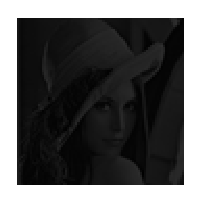
\includegraphics[scale=0.7]{SprecherPics/Couche1.eps}\\Première couche \\($g_0(\xi)$)\end{center}\end{minipage}$+ \cdots +$
	\begin{minipage}[c]{2.3cm}\begin{center}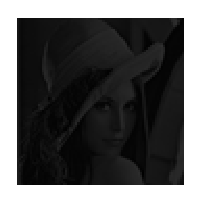
\includegraphics[scale=0.7]{SprecherPics/Couche1.eps}\\Cinquième couche\\($g_4(\xi)$) \end{center}\end{minipage} $=$
	\begin{minipage}[c]{2.3cm}\begin{center}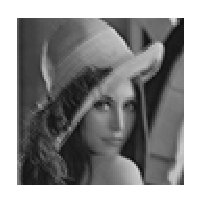
\includegraphics[scale=0.7]{SprecherPics/Reconstitution1.eps}\\Reconstitution après une itération \end{center}\end{minipage}
	\end{center}
\end{frame}
\begin{frame}
	\titp{L'algorithme de Sprecher :}
	$\phi$ et $\xi$ pour l'algorithme de Sprecher : \hspace{1cm}	
	\begin{minipage}[c]{2.3cm}\begin{center}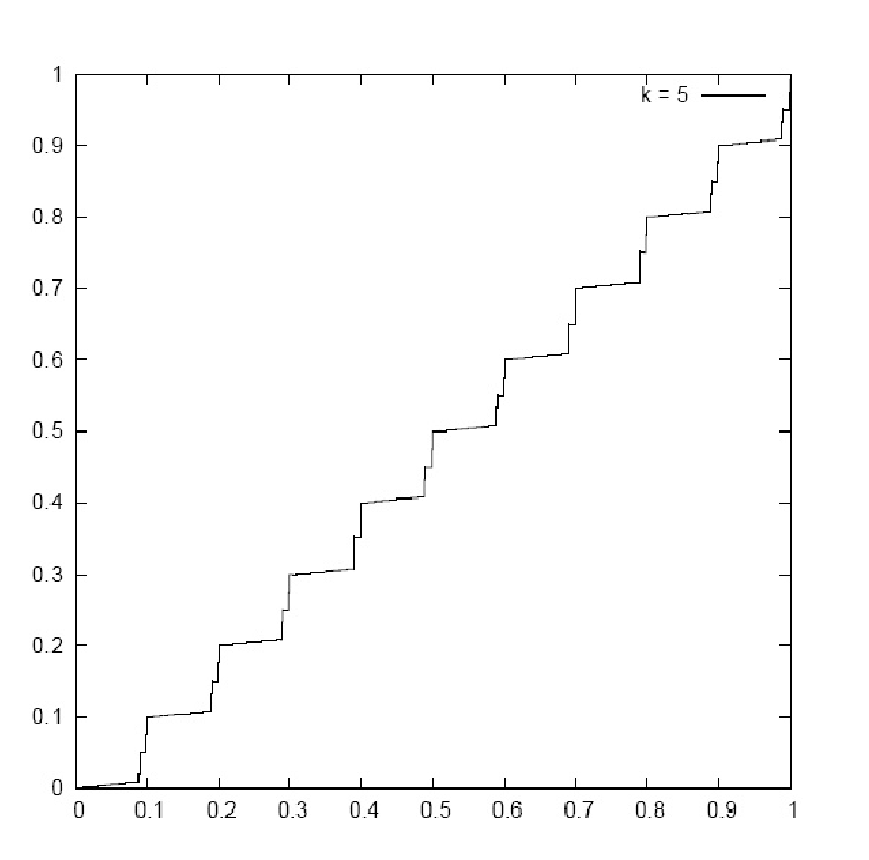
\includegraphics[scale=0.15]{SprecherPics/Psi.eps}\\$\phi$ sur $[0,1]$ \end{center}\end{minipage} $\Rightarrow$
	\begin{minipage}[c]{2.6cm}\begin{center}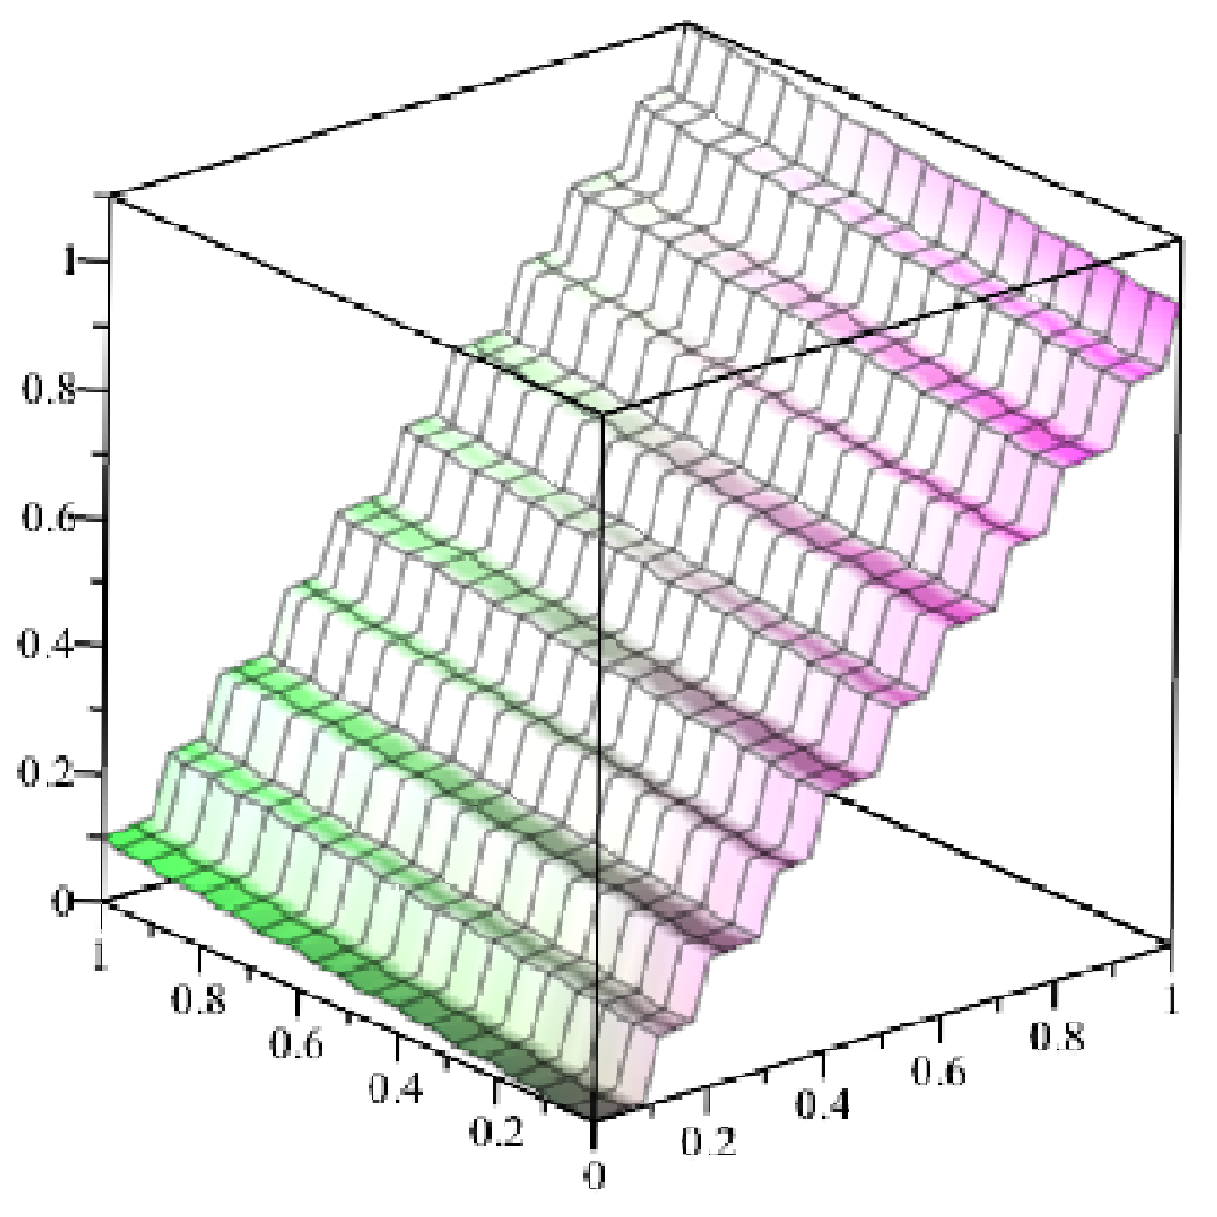
\includegraphics[scale=0.15]{SprecherPics/Xi.eps}\\$\xi$ sur $[0,1]^2$ \end{center}\end{minipage}\\
	\begin{center} $\displaystyle f(x, y) = \lim\limits_{r \to \infty} \sum\limits_{n=0}^{4} \underbrace{\sum\limits_{j=1}^{r} g_{n,j} \circ \xi(x+n b, y + n b)}_{g_n\left(\xi(x+n b, y + n b)\right)}$ \end{center}
\end{frame}

\subsection{Les résultats}
\begin{frame}
	\titp{Le stockage des fonctions :}
	Les $\lambda_i$ et $\phi$ sont indépendantes de l'image.\\
	On ne stocke que les $(g_i)_{i\in\lbrace 0,…,2d\rbrace} \hspace{1cm}\xrightarrow{\text{Discrétisation}}$ $n*(2\times d + 1)$ points à enregistrer.
	\textbf{\\}
	\begin{center}
	\begin{tabular}{rccc}
	\hline
	 & Image originale&\vline &Algorithme de Sprecher \\
	Quantité de données :& $n^2$ points & $\xrightarrow{\text{Kolmogorov}}$& $50\times n$ valeurs\\
	Complexité :& $O(n^2)$& $\xrightarrow{\text{Kolmogorov}}$& $O(n)$\\\hline
	\end{tabular}
	\end{center}
	\renewcommand{\arraystretch}{1.5}
	\setlength\doublerulesep{3pt}
	\textbf{\\}\textbf{\\}
	\titp{Comparaison des différents formats}
	\small{
		\begin{tabular}{c|c|c}
			$40\times 40$ & $128\times 128$ & $500\times 500$ \\
		\hline
			\cellcolor{vertpale}  \textbf{BMP} : 1.56Ko \textit{(1600 octets)} &\cellcolor{rougepale} \textbf{BMP} : 16.0Ko \textit{(16384 octets)}&\cellcolor{rougepale} \textbf{BMP} : 244.14Ko \textit{(250000 octets)}\\
		\hline
			\cellcolor{jaunepale} \textbf{TSK} : 1.93Ko \textit{(2000 octets)} &\cellcolor{jaunepale} \textbf{TSK} : 6.25Ko \textit{(6400 octets)}&\cellcolor{vertpale} \textbf{TSK} : 24.14Ko \textit{(25000 octets)}\\
		\hline
			\cellcolor{rougepale} \textbf{JPG} : 11.8Ko \textit{(12158 octets)}&\cellcolor{vertpale} \textbf{JPG} : 4.38Ko \textit{(4491 octets)}&\cellcolor{jaunepale} \textbf{JPG} : 49.2Ko \textit{(50396 octets)}\\
		\end{tabular}}
\end{frame}
\section*{Conclusion}
\begin{frame}
	\titp{Conclusion}
	\begin{enumerate}
		\item Un puissant outil d'analyse et de traitement du signal
		\item Une démonstration non-constructive simple
		\item Peu de mises en application à ce jour…
		\item Permet un taux de compression très élevé pour de grands échantillons de données
		\item A un avenir prometteur (Vidéo,…)
	\end{enumerate}
\end{frame}
\end{document}

\begin{block}{Théorème de Superposition de Kolmogorov}
\begin{center}
$ \forall n \in \mathbb{N}, $
$\exists \phi_1, …, \phi_n$\\ \textbf{telles que}\\

Pour $ f \in \mathcal{C}^o([0,1]^n, \mathbb{R})$ \emph{quelconque},\\

$\exists g_1,…,g_{2n+1} \in \mathcal{C}^o(\mathbb{R},\mathbb{R})$\\ \textbf{telles que}

\end{center}
\[f(x_1,…,x_n)= \sum\limits_{q=1}^{2n+1} g_q\left(\sum\limits_{p=1}^{n}\phi_{p,q}(x_p)\right) \]

\end{block}
	Comme souvent en mathématiques et en physique, la dimension est source de difficultés.\\
	Plus la dimension est grande, plus les phénomènes mathématiques et physiques sont compliqués.
